%%
%% 2019 07 04 Ph. G. Freimann
%%

\section{Zahlen}
\sectuntertitel{Im 15. Jahrhundert --- genauer im Jahre 1413 --- am
  zwölften elften um zehn Uhr neun haben acht der sieben Schlauesten
  gesagt: ``So sechs wie wir fünf gibt's keine vier mehr, denn wir
  drei sind die zwei einzigen Nullen.``}



%%\TALSTadBFWA{8}{1.1}
%%%%%%%%%%%%%%%%%%%%%%%%%%%%%%%%%%%%%%%%%%%%%%%%%%%%%%%%%%%%%%%%%%%%%%%%%%%%%%%%%
\subsection*{Lernziele}

\begin{itemize}
	\item Zahlmengen $\mathbb{N}$, $\mathbb{Z}$, $\mathbb{Q}$, $\mathbb{R}$
  \item Näherungswerte, Runden
  \item Wissenschaftliche Notation
  \item Ordnungsrelationen ($=$, $<$, $>$, $\leq$, $\geq$)
  \item Betrag
\end{itemize}

\TadBMTA{13}{1.1}

\newpage

\subsection{Die natürlichen Zahlen ($\mathbb{N}$)}\index{Zahlen!natürliche}

\begin{definition}{natürliche Zahlen}{definition_natuerliche_zahlen}
  Natürliche Zahlen $\mathbb{N}$ sind ganze positive Zahlen: ${1, 2, 3, 4, 5, ....}$.
\end{definition}

\TALS{
  \begin{bemerkung}{Null}{}
  Selten wird auch die Menge ${0, 1, 2, 3, 4, ...}$ als die Menge
  der natürlichen Zahlen bezeichnet. Wenn die Unterscheidung
  wesentlich ist, verzichten wir auf die Schreibweise $\mathbb{N}$ und
  verwenden

  $$\mathbb{N}_0 = \mathbb{N}\cup{} \{0 \}  = \{0, 1, 2, 3, 4, ...\}$$
  bzw.
  $$\mathbb{N}\backslash\{0\} =\mathbb{N}^\ast= \mathbb{N}^+= \{1, 2, 3, 4, ...\}.$$
  \end{bemerkung}
}%% END TALS

\GESO{\begin{bemerkung}{Notation}{}
  Um explizit anzugeben, dass die Zahl Null nicht zu $\mathbb{N}$ gehört schreiben wir:
  $$\mathbb{N}\backslash{}\{0\}$$
  Um explizit anzugeben, dass die Zahl Null zur Menge $\mathbb{N}$ gehören soll, schreiben wir:
  $$\mathbb{N}_0$$
\end{bemerkung}}%% END GESO


Mit natürlichen Zahlen können wir beliebig
\begin{itemize}
\item \textbf{addieren} ($+$)  und
\item \textbf{multiplizieren} ($\cdot{}$).
\end{itemize}


\TALS{\newpage}


\subsection{Ganze Zahlen ($\mathbb{Z}$)}\index{Zahlen!ganze}
\begin{definition}{ganze Zahlen}{definition_ganze_zahlen}

  Mit $\mathbb{Z}$ bezeichnen wir alle ganzen Zahlen, sowohl die
  positiven ($\mathbb{N}$), wie auch die negativen.
  \end{definition}

$$\mathbb{Z} = \{..., -3, -2, -1, 0, 1, 2, 3,  4, ... \}$$

Zusätzlich zu den natürlichen Zahlen können wir nun eine
\begin{itemize}
\item \textbf{Subtraktion} ($-$)
  \end{itemize}
uneingeschränkt durchführen.

\TALS{
\subsubsection{Zahlenstrahl / Zahlengerade}\index{Zahlenstrahl}

\begin{center}
\raisebox{-1cm}{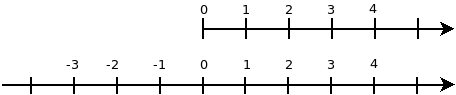
\includegraphics[width=13cm]{allg/alg/img/Zahlenstrahl.png}}
\end{center}

Der Zahlenstrahl hat den Startpunkt 0 (Null)\footnote{... manchmal  den Startpunkt 1 ...}, wohingegen die
Zahlengerade auf beiden Seiten uneingeschränkt weiterläuft.}%% END TALS
\newpage


\subsection{Rationale Zahlen ($\mathbb{Q}$)}
\index{Zahlen!rationale}\index{rationale Zahlen}

\begin{definition}{rationale Zahlen}{}
Zahlen, welche sich als Bruch mit ganzen Zahlen schreiben lassen,
werden als \textbf{rationale Zahlen} bezeichnet.


$$\mathbb{Q} =\left\{ q = \frac{a}{b} \,\,\, \middle| \,\,\, a \in \mathbb{Z}, b \in \mathbb{N}\backslash{}\{0\}\right\}$$
\end{definition}

\subsubsection{Dezimalbrüche}\index{Dezimalbruch}
Jeder Bruch ($\frac{a}{b}$\TRAINER{  $a, b \in \mathbb{Z}, b\ne 0$}) lässt sich als
abbrechender oder periodischer Dezimalbruch schreiben. Beispiel:

Abbrechend:
$$\frac{175}{8} = \LoesungsRaumLang{21.875}$$
Periodisch:
$$\frac{5}{70} = \LoesungsRaumLang{0.0\overline{714285}}$$

Dasselbe gilt umgekehrt. Für abbrechende Dezimalbrüche ist dies
trivial:
$$47.386 = \LoesungsRaumLang{\frac{47\,386}{1\,000}}$$

Für periodische, nicht abbrechende
Dezimalbrüche\index{Dezimalbruch!periodisch}\index{periodische Dezimalbrüche} sieht die Sache etwas komplizierter aus,
gilt jedoch auch (sprich «Null Komma Periode Eins-Drei»):

$$0.\overline{13} = 0.131313... = \LoesungsRaumLang{13\cdot{}\frac1{99}=\frac{13}{99} = 13 : 99}$$

\TNTeop{Bem.: $\frac{1}{9} = 0.111\overline{1}$, $\frac{1}{99} = 0.0101\overline{01}$, $\frac{1}{999} = 0.001001\overline{001}$, ...}

%%%%%%%%%%%%%%%%%%%%%%%%%%%%%%%%%%%%%%%%%%%%

  \subsection*{Aufgaben}
  Zeigen Sie, dass die folgenden Dezimalzahlen rational sind. Schreiben Sie dazu diese Zahlen als gewöhnliche, gekürzte Brüche:

  \renewcommand{\arraystretch}{1.5}
  \begin{tabular}{|c|c|c|}
  $0.8=\LoesungsRaum{\frac45}$                  & $-2.03=\LoesungsRaum{-\frac{203}{100}}$         & $2.125=\LoesungsRaum{\frac{17}{8}}$                             \\
  $3.\overline{3}=\LoesungsRaum{\frac{10}{3} }$ & $4.\overline{16}=\LoesungsRaum{\frac{412}{99}}$ & $1.\overline{538461} =\LoesungsRaum{\frac{170\,940}{111\,111}}$ 
  \end{tabular} 
  \renewcommand{\arraystretch}{1}


\TNTeop{}

%%  \GESOAadBMTA{22}{Optional: 6., 7.}
%%  \TALSAadBMTA{8}{Optional: 1., 2.}

%%  \noTRAINER{\mmPapier{6}}%% END noTRAINER

%%%%%%%%%%%%%%%%%%%%%%%%%%%%%%%%%%%%%%%%%%%


\subsection{Runden}\index{runden}
In der Regel sind wir bei Dezimalbrüchen nicht an allen auftretenden
Stellen interessiert, sondern begnügen uns mit einer Näherung.

\subsubsection{Dezimalen (Nachkommastellen)}\index{Dezimale}\index{Nachkommastelle}
Als Dezimalen, Dezimalstellen oder Nachkommastellen werden die Stellen
\textbf{nach} dem Komma bezeichnet.

\begin{rezept}{Runden}{}
  Beim \textbf{Runden} auf die $n$-te Stelle, wird die $n+1$-te Stelle
  betrachtet. Ist diese >=5, so wird \textbf{aufgerundet}, ansonsten \textbf{abgerundet}.
\end{rezept}

Runden auf die vierte \textbf{Dezimale} (= vierte \textbf{Nachkommastelle}):
$$ 36.4699432 \approx  \LoesungsRaum{36.4699}$$
$$ 36.4699618 \approx  \LoesungsRaum{36.4700}$$
\textbf{Vorsicht} bei Zahlen nahe an Null. So wird die Zahl
$$0.002468$$ beim Runden auf vier Dezimalen wie folgt gerundet:
$$0.0025$$

Runden Sie auf {\color{ForestGreen}vier} Dezimalen:

\begin{tabular}{rcl}
  $55.55555$      &$\approx$& \LoesungsRaum{$55.{\color{ForestGreen}\mathbf{5556}}$}\\
  $8.55695$       &$\approx$& \LoesungsRaum{$8.{\color{ForestGreen}\mathbf{5570}}$}\\
  $3.3339499$     &$\approx$& \LoesungsRaum{$3.{\color{ForestGreen}\mathbf{3339}}$}\\
  $1000.0001$     &$\approx$& \LoesungsRaum{$1000.{\color{ForestGreen}\mathbf{0001}}$}\\
  $10\,000.00001$ &$\approx$& \LoesungsRaum{$10\,000.{\color{ForestGreen}\mathbf{0000}}$}\\
  $-6.99999$      &$\approx$& \LoesungsRaum{$-7.{\color{ForestGreen}\mathbf{0000}}$}\\
  $0.000040447$   &$\approx$& \LoesungsRaum{$0.{\color{ForestGreen}\mathbf{0000}}$}\\
\end{tabular}

\TRAINER{Das letzte Beispiel zeigt, dass so oft wichtige Information
  verloren geht. Daher wird sinnvollerweise meist auf signifikante Stellen, und nicht
  auf Dezimalen gerundet.}
\newpage

\subsubsection{Signifikante Stellen\GESO{ (optional)}}\index{signifikante Stellen}
\begin{rezept}{Auf signifikante Ziffern runden}{}
  
  Beim Runden auf \textbf{vier signifikante Ziffern} wird
  \begin{itemize}
  \item  von links nach rechts die erste von Null verschiedene Ziffer gesucht. Dies ist die
    erste signifikante Ziffer.
  \item
    Danach werden die nächsten drei Ziffern
  genommen, egal ob sie Null sind oder nicht. 
\item   Mit diesen drei Ziffern bilden die Ziffern zusammen die vier
  signifikanten Ziffern.
\item  Die 5. Ziffer wird nur noch zum Auf- oder Abrunden verwendet.
  \end{itemize}
\end{rezept}

Geben Sie {\color{ForestGreen}\textbf{vier}} \textbf{signifikante} Ziffern an und runden Sie wenn nötig:

$$0.000040447  \approx \LoesungsRaum{0.0000{\color{ForestGreen}\mathbf{4045}}}$$
$$36.4699432 \approx \LoesungsRaum{{\color{ForestGreen}\mathbf{36.47}}}$$
$$36.9952831 \approx \LoesungsRaum{{\color{ForestGreen}\mathbf{37.00}}}$$
$$30009.78   \approx \LoesungsRaum{{\color{ForestGreen}\mathbf{3001}}0}$$
$$0.0439899  \approx \LoesungsRaum{0.0{\color{ForestGreen}\mathbf{4399}}}$$
$$1\,000\,000 \approx \LoesungsRaum{{\color{ForestGreen}\mathbf{1\,000}}\,000}$$
$$0.00001    \approx \LoesungsRaum{0.0000{\color{ForestGreen}\mathbf{1000}}}$$


\subsection*{Aufgaben}

\aufgabenFarbe{Runden Sie die Zahl 3.21459 auf zwei Dezimalen: \LoesungsRaumLang{3.21}. Runden Sie die selbe Zahl 3.21459 auf drei Dezimalen: \LoesungsRaumLang{3.215} und runden Sie nun das gerundete Resultat auf zwei Dezimalen: \LoesungsRaumLang{3.22}. Was ist davon zu halten?}%% END Aufgabenfarbe

\TNTeop{Rechnen Sie nie mit bereits gerundeten Zwischenresultaten. Der Fehler kann sich dadurch vergrößern!}%% END TNT

%%%%%%%%%%%%%%%%%%%%%%%%%%%%%%%%
  
\subsubsection{Wissenschaftliche Notation}\index{Notation!wissenschaftliche}\label{wissenschaftlicheNotation}
Bei Zahlen größer als 10 können wir einer Zahl manchmal nicht ansehen, wie viel Stellen denn nun signifikant sind.

$$ 679\,946 \textrm{\ Einwohner} \approx  \LoesungsRaumLang{680\,000} \textrm{\ Einwohner}$$
$$ 680\,023 \textrm{\ Einwohner} \approx  \LoesungsRaumLang{680\,000} \textrm{\ Einwohner}$$

Daher bietet sich die wissenschaftliche Notation an.\footnote{Die
\textbf{wissenschaftliche Notation} wird vorwiegend für sehr große
aber auch für Zahlen sehr nahe an Null verwendet.}
Bei der wissenschaftlichen Notation wird die erste signifikante Ziffer
vor das Komma geschrieben. Nach dem Komma stehen \textbf{alle} weiteren signifikanten Stellen.
Zuletzt wird die Zahl mit Zehnerpotenzen
($10^{n}: n \in \mathbb{Z}$) «an die richtige Stelle» gerückt:

$$64\,038.6  = \LoesungsRaumLang{6.40386 \cdot 10^{ 4}} \approx \LoesungsRaumLang{6.40 \cdot 10^{ 4}}$$
$$0.00463640 = \LoesungsRaumLang{4.63640 \cdot 10^{-3}} \approx \LoesungsRaumLang{4.64 \cdot 10^{-3}}$$

Dabei bezeichnen negative Exponenten die Zehntel, Hundertstel, etc.
Erst in der wissenschaftlichen Notation können wir die signifikanten Stellen auch bei gerundeten Zahlen größer als 10 effektiv ablesen.


Stellen Sie in Wissenschaftlicher Notation dar:

0.00479 $= \LoesungsRaum{4.79 \cdot{}10^{-3}}$

0.08 Milliarden $= \LoesungsRaum{8\cdot{}10^7}$

%%\TALS{S. \cite{frommenwiler17alg} S. 40 Kap. 1.5.5}
\newpage

\paragraph{Taschenrechner} Auf Taschenrechnern oder in
Programmiersprachen wird die Exponentialschreibweise i.\,d.\,R. mit dem
Buchstaben «e» angegeben. Also «e$\color{red}n$» anstelle von «$\cdot10^{\color{red}n}$». Beispiele:

$5\,000 = 5\, \cdot 10^{\color{red}3} = 5\mathrm{e}\color{red}3$

$0.063 = 6.3\, \cdot 10^{-2} = 6.3\mathrm{e-}2$

Interpretieren Sie:

\leserluft{}

$$0.0123e3 = \LoesungsRaumLang{12.3}$$

\leserluft{}

$$14150.333e-3 =\LoesungsRaumLang{14.150333}$$


Berechnen Sie (und überprüfen Sie mit dem Taschenrechner):

$$5.7^{15} = \LoesungsRaumLang{2.178e11} = \LoesungsRaumLang{2.178 \cdot{} 10^{11}}$$
$$0.44^{28} =\LoesungsRaumLang{1.039e-10} = \LoesungsRaumLang{1.039\cdot{} 10^{-10}}$$
\begin{rezept}{EE}{}
    Um 5.77 Millionen auf Ihrem Taschenrechner \textbf{einzugeben} tippen Sie:

\begin{center}  \TRAINER{5.77 \GESO{\tiprobutton{EE}}\TALS{\nspirebutton{EE}} 6}\noTRAINER{\vspace{5mm}} \end{center}

\end{rezept}
\GESO{\begin{rezept}{SCI}{}
   Der Taschenrechner kann auch direkt die \textit{Wissenschaftliche Notation}
   anzeigen, wenn er so eingestellt ist:

   Beispiel 0.087 in \textit{Wissenschaftlicher Notation}:

   0.087 \tiprobutton{mode}\texttt{SCI}\tiprobutton{enter}\tiprobutton{2nd}\tiprobutton{mode_quit}\tiprobutton{enter}

   \texttt{8.7E-2} (Dies bedeutet $8.7 \cdot{} 10^{-2}$.)
\end{rezept}
}%% END GESO
\newpage

\subsection{Irrationale und reelle Zahlen ($\mathbb{R}$)}\index{Zahlen!reelle}

\youtubeLink{https://www.youtube.com/watch?v=9JgcETAN65c}{Simple-Club:
  Irrationale Zahlen}

\youtubeLink{https://www.youtube.com/watch?v=tPfnEByx9r0}{Dorfuchs: Wurzel zwei ist irrational.}

  Zahlen auf der Zahlengerade, welche nicht als Bruch $\frac{a}{b}$ mit $a\in\mathbb{Z}$, $b \in \mathbb{N}$ dargestellt werden können, werden als \textbf{irrational}\index{irrational} bezeichnet.

Wichtigste Vertreter:

\TNT{5.2}{\bbwCenterGraphic{12cm}{allg/alg/img/IrrationaleZahlen.png}}

\begin{definition}{Reelle Zahl}{}
Die Vereinigungsmenge der rationalen ($\mathbb{Q}$) und der irrationalen Zahlen
nennen wir die \textbf{reellen} Zahlen und bezeichnen die Menge mit $\mathbb{R}$.
\end{definition}


Dass $\pi$ oder $\sqrt{2}$ irrational sind, ist nicht trivial. Daher
noch zwei Vertreter irrationaler Zahlen, bei denen sofort klar ist,
dass es sich nicht um periodische Dezimalbrüche handelt:
\TNTeop{\begin{itemize}
\item $0.10 100 100010000100000100000010000000...$
\item $0.12345678910111213141516 ... 9899100101102103104 ... $
\end{itemize}%%
}%% END TNT

%%%%%%%%%%%%%%%%%%%%%%%%%%%%%%%%%%%%%%%%%%%%

\begin{gesetz}{Zahlmengen Beziehungen}{}
$$\LoesungsRaum{\mathbb{N}} \subset \LoesungsRaum{\mathbb{Z}} \subset
  \LoesungsRaum{\mathbb{Q}} \subset \LoesungsRaum{\mathbb{R}} $$%
\end{gesetz}


\begin{bemerkung}{Mächtigkeit}{}
  Dabei ist $\mathbb{R}$ die mächtigste der vier Mengen. 
\end{bemerkung}

\TNTeop{(Trainer: Beginne beim skizzieren mit $\mathbb{R}$)\\
\bbwCenterGraphic{8cm}{allg/alg/img/nzqr.png}
}%% END TNTeop

%%%%%%%%%%%%%%%%%%%%%%%%%%%%%%%%%%%%%%

\subsection*{Aufgaben zum Kapitel Zahlmengen}

\aufgabenFarbe{Geben Sie jeweils an, zu welchen der Zahlmengen $\mathbb{N}\backslash{}\{0\}$, $\mathbb{Z}$, $\mathbb{Q}$ bzw. $\mathbb{R}$ die folgenden Zahlen gehören:%%
}%% END Aufgabenfarbe

\begin{itemize}
\item $5-8 \LoesungsRaum{\mathbb{Z,Q,R}}$
\item $-3.\overline{17} \LoesungsRaum{\mathbb{Q,R}}$
\item $\sqrt{2.00} - \sqrt{\frac{50}{25}} \LoesungsRaum{\mathbb{Z,Q,R}}$
\item $\frac{3}{\pi} \LoesungsRaum{\mathbb{R}}$
\item $\sqrt{2^5}\LoesungsRaum{\mathbb{R}}$
\item $4.\overline{9} \LoesungsRaum{\mathbb{N,Z,Q,R}}$
\item $3.\overline{18}+\frac{20}{11} \LoesungsRaum{\mathbb{N,Z,Q,R}}$
\item $0.313113111311113111113... \LoesungsRaum{\mathbb{R}}$
\item $\sqrt{-6} \LoesungsRaum{\not\in\mathbb{R}}$
\end{itemize} 

%%\GESOAadBMTA{22ff}{5.}
%%\TALSAadBMTA{9}{4.}

\TNTeop{}
